\documentclass[tikz,border=7pt]{standalone}
\usepackage{amsmath,amssymb,pgfplots}
\pgfplotsset{compat=1.18}
\usetikzlibrary{arrows.meta}
\begin{document}
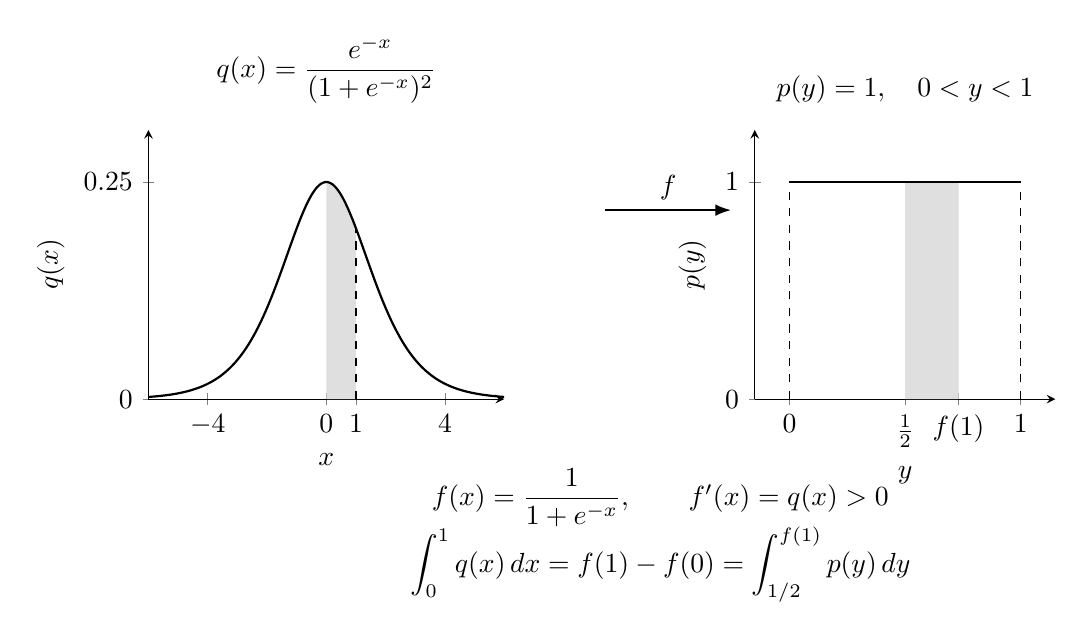
\begin{tikzpicture}
\begin{axis}[name=src,width=6.1cm,height=5cm,xmin=-6,xmax=6,ymin=0,ymax=.31,
axis lines=left,xlabel={$x$},ylabel={$q(x)$},xtick={-4,0,1,4},ytick={0,.25},
title={$q(x)=\dfrac{e^{-x}}{(1+e^{-x})^2}$},samples=180]
\addplot[draw=none,fill=gray!25,domain=0:1] {exp(-x)/(1+exp(-x))^2}\closedcycle;
\addplot[thick,domain=-6:6] {exp(-x)/(1+exp(-x))^2};
\addplot[dashed] coordinates {(1,0) (1,.19661193)};
\end{axis}
\begin{axis}[at={(7.7cm,0)},anchor=south west,name=dst,width=5.4cm,height=5cm,
xmin=-.15,xmax=1.15,ymin=0,ymax=1.24,axis lines=left,
xlabel={$y$},ylabel={$p(y)$},xtick={0,.5,.73105858,1},xticklabels={$0$,$\frac12$,$f(1)$,$1$},
ytick={0,1},title={$p(y)=1,\quad 0<y<1$}]
\addplot[draw=none,fill=gray!25] coordinates {(.5,0) (.5,1) (.73105858,1) (.73105858,0)}\closedcycle;
\addplot[thick] coordinates {(0,1) (1,1)};
\addplot[dashed] coordinates {(0,0) (0,1)};
\addplot[dashed] coordinates {(1,0) (1,1)};
\end{axis}
\draw[-{Latex[length=2mm]},thick] (5.8,2.4) -- (7.4,2.4)
node[midway,above] {$f$};
\node at (6.5,-1.25) {$f(x)=\dfrac{1}{1+e^{-x}},\qquad f'(x)=q(x)>0$};
\node at (6.5,-2.1) {$\displaystyle\int_0^1q(x)\,dx=f(1)-f(0)=\int_{1/2}^{f(1)}p(y)\,dy$};
\end{tikzpicture}
\end{document}
